\subsection{Fit dos tempos entre chegadas para cada mês} 
\label{section: fit-arrivals}
Conforme atestado no teste de hipóteses apresentado na Figura \ref*{fig: ks-arrivals}, o tempo entre as chegadas das ligações muda mês a mês, sendo necessário representar o intervalo entre as chegadas com diferentes distribuições de probabilidade ao longo do tempo em nosso modelo de simulação. A distribuição exponencial é a mais adequada para modelar os dados em todos os meses, visto que apresenta pequenos erros e maiores valores $p$ em relação às demais distribuições.

\subsubsection*{Janeiro}
No primeiro mês do ano, o teste de aderência de Kolgomogorov-Smirnov indica que a distribuição que melhor representa os valores dos tempos entre chegadas é a exponencial com média 248,6240 segundos. A Figura \ref*{fig: fit-janeiro} apresenta o resumo dos testes realizados.

\begin{figure}[H]
    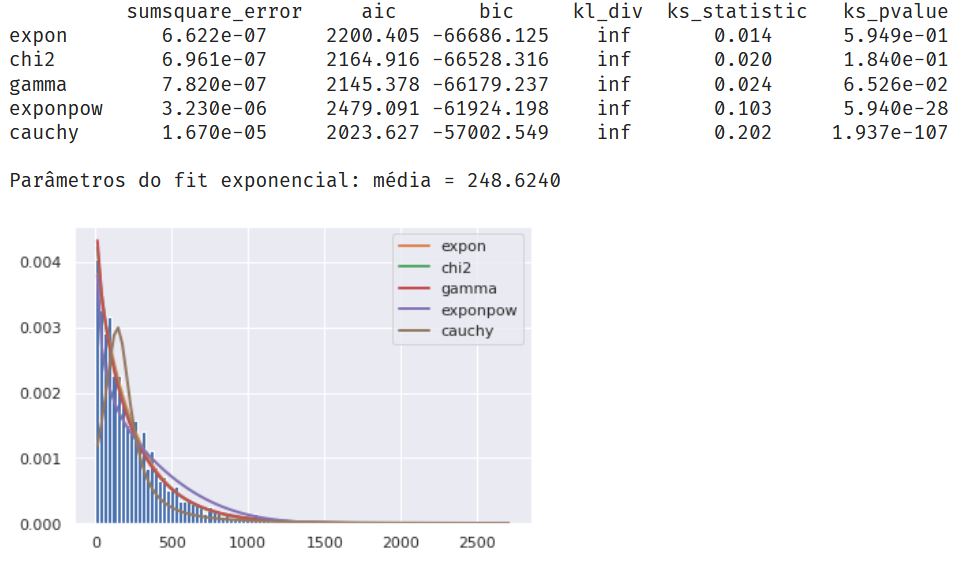
\includegraphics[scale=0.8]{analise-de-dados/fit/fit-janeiro.png}
    \caption{Teste de aderência dos tempos entre chegadas para o mês de janeiro}
    \label{fig: fit-janeiro}
\end{figure}

\subsubsection*{Fevereiro}
\subsubsection*{Março}
\subsubsection*{Abril}
\subsubsection*{Junho}
\subsubsection*{Julho}
\subsubsection*{Agosto}
\subsubsection*{Setembro}
\subsubsection*{Outubro}
\subsubsection*{Novembro}
\subsubsection*{Dezembro}